\subsection{What if an LLM reads the news?}

One may wonder whether clustering news articles based on a deeper understanding of their content could lead to a more profitable trading strategy. For this purpose, we feed the news articles to a Large Language Model (LLM) and ask it to analyze them according to a predefined schema.

%%%%%%%%%%%%%%%%%%%%%%%%%%%%%%%%%%%%%%%%%%%%%%%%%%%%%
%%%%%%%%%%%%%%%%%%%%%%%%%%%%%%%%%%%%%%%%%%%%%%%%%%%%%
\subsubsection{Large Language Models}

In natural language processing (NLP), Large Language Models (LLMs) are designed to \qquote{understand} and generate human-like text. These models utilize the transformer architecture, which excels in modeling complex language tasks by capturing long-range dependencies and contextual relationships.

\mx 
At the heart of LLMs lies the concept of tokens, which serve as the elemental units of text. Tokens can be individual words, subword units, or characters. Let $x_{1:n}:=\3{x_1, x_2, \ldots, x_n}$ represent a sequence of tokens. The goal of an LLM is to estimate the probability distribution of the next token $x_{n+1}$ conditioned on the previous tokens $x_{1:n}$
$$
\P\2{x_{n+1} \mid \3{x_1, x_2, \ldots, x_n}}
.
$$

%\mx 
An LLM is a neural network architecture designed to learn and approximate this conditional probability distribution over sequences of tokens with a large number of parameters $\Theta$. Namely, we can formulate an LLM as a parameterized function $f_{\Theta}$ that maps a sequence of tokens $\3{x_1, x_2, \ldots, x_n}$ to a probability distribution over the vocabulary, where the parameters $\Theta$ are learned from a large corpus of text training data.
$$
f_{\Theta}:\3{x_1, x_2, \ldots, x_n} \rightarrow 
\P\2{x_{n+1} \mid \3{x_1, x_2, \ldots, x_n} ; \Theta}
$$

%\mx 
Interacting with an LLM involves specifying a prefix sequence $x_{1:n}$, termed the \qquote{prompt}, and sampling the subsequent tokens $x_{n+1:z}$, known as the \qquote{completion}. This process enables users to guide and control the generation of text according to desired contexts and constraints.
$$
\ub{\3{x_1,\ldots,x_n}}{\t{prompt}} \longrightarrow \ub{\3{x_{n+1},\ldots,x_z}}{\t{completion}}
$$


\subsubsection{Evolution of LLMs}
\hspace{0.5cm} The transformer architecture, introduced in the seminal work "Attention Is All You Need" \citep{vaswani2017attention}, revolutionized LLM development due to its superior handling of long-range dependencies and efficient parallelization of computations.  Subsequent advancements include the encoder-only BERT model \citep{devlin2018bert}, showcasing the power of pre-training on large datasets for fine-tuning on specific tasks. 

\mx 
Conversely, OpenAI's GPT series (\citealp{radford2018improving}) demonstrated the potential of decoder-only models for generative tasks. In particular, the release of GPT-3 marked a significant leap in LLM capabilities with its 175 billion parameters and remarkable few-shot learning abilities. This model highlighted the importance of prompt engineering, where carefully crafted prompts can guide model outputs without extensive fine-tuning.  

\mx 
The trend towards open-source models like BLOOM \citep{le2023bloom} and Meta's LLaMA series \citep{touvron2023llama} emphasizes accessibility and transparency in LLM development.  The latest models, including OpenAI's GPT-4 and GPT-4o, Google's Gemini, and Meta's LLaMA 3 and 3.1 continue to push boundaries with improved accuracy, multimodal capabilities, and larger context windows.

%The transformer architecture presented in the seminal paper "Attention Is All You Need" in 2017 became the foundation for most subsequent LLMs due to its superior ability to handle long-range dependencies and parallelize computations.  The introduction of BERT in 2018, an encoder-only model, demonstrated the power of pre-training on large text corpora and fine-tuning for specific tasks. In contrast, OpenAI's GPT series, starting with GPT-1 in 2018 and gaining widespread attention with GPT-2 in 2019, showcased the capabilities of decoder-only models for generative tasks.
%
%The release of GPT-3 in 2020 marked a significant leap with 175 billion parameters, demonstrating remarkable few-shot learning capabilities. This model highlighted the potential of prompt engineering to guide model outputs without extensive fine-tuning.
%
%From 2022 onwards, source-available models like BLOOM and Meta's LLaMA series have emphasized the importance of accessibility and transparency in LLM development. The latest models, such as OpenAI's GPT-4o, Google's Gemini, and Meta's LLaMA 3, continue to push the boundaries with improved accuracy, multimodal capabilities, and larger context windows, solidifying the transformer architecture as the standard for LLMs.

\subsubsection{Function Calling with LlaMA-3}

\hspace{0.5cm} In our endeavor we will employ LlaMA-3, developed by Meta AI and released on April 18, 2024. This model has been pre-trained on approximately 15 trillion tokens of text gathered from ``publicly available sources'' and it comes in two sizes: 8 billion and 70 billion parameters. In this application, we will employ the 70B version, which we will access through an API via GroqCloud.

\mx 
Moreover, we will employ a \textit{function calling} approach to streamline the process of interacting with the LLM. This implies prespecifying a set of functions to the LLM that will then be passed through our dataset of news articles to obtain a structured output in JSON format. The formal procedure is thoroughly described in the Appendix (\cref{alg:function_calling}).

\mx 
Each article $i\in\D$ implies a conversation with the LLM. The structure of the conversation implies defining first a ``system message'', which provides a general context and purpose to the model. In our case:

\begin{quote}
\textit{$-$ You are a function calling LLM that analyses business news in Spanish.  \\
$-$ For every article, you must identify the firms directly affected by the news. Do not include every firm mentioned in the article, only include those that are directly affected by the shocks narrated therein. 
\\
$-$ The identified firms must be Spanish and should be publicly listed in the Spanish exchange (their ticker is of the form 'TICKER.MC'). Do not include non-Spanish foreign firms. Do not include Spanish firms that are not publicly traded. \\
$-$ For each identified firm, classify the shocks that affect them (type, magnitude, category). The type of shock can be 'demand', 'supply', 'financial', 'policy', or 'technology'. The magnitude can be 'minor' or 'major'. The direction can be 'positive' or 'negative'. \\
$-$ If a firm is affected neutrally by the news article, don't include it in the analysis.
}
\end{quote}

Then, a news article is fed to the LLM, for example:

\begin{quote}

{\centering 
\textbf{Cellnex tendr� m�s competencia en Europa}.  \par }
\textit{
La filial de Telef�nica (TEF.MC) Telxius Telecom ha acordado vender su divisi�n de torres de telecomunicaciones en Europa y Latinoam�rica a American Tower (AMT), lo cual aumentar� la presencia de �sta en Europa e incrementar� la competencia para el grupo espa�ol de telecomunicaciones inal�mbricas Cellnex Telecom (CLNX.MC), se�ala Equita Sim. La transacci�n "supone la entrada de un nuevo operador independiente de torres en el mercado espa�ol y potencialmente m�s competencia para el crecimiento futuro tambi�n en el mercado europeo", sostiene la corredur�a. 
%Cellnex lleg� a un acuerdo en noviembre con CK Hutchison (0001.HK) para comprar el negocio europeo de torres y sus activos del conglomerado cotizado en Hong Kong. La acci�n de Telef�nica sube un 9,6\% a EUR3,94 y la de Cellnex avanza un 0,3\% a EUR47,79.
}
\end{quote}
%\begin{quote}
%{\centering \textbf{Permanencia de los Benetton en accionariado Cellnex ser�a positiva}. \par }
%\textit{
%En medio de las especulaciones en prensa sobre el inter�s de varios fondos internacionales por la participaci�n de los Benetton en Cellnex (CLNX.MC), Banco Sabadell cree que la permanencia de la familia italiana en el accionariado del operador espa�ol de infraestructuras de telecomunicaciones ser�a doblemente positiva. Por un lado, el compromiso de los Benetton con el proyecto de Cellnex alejar�a el riesgo de una posible presi�n vendedora en el corto plazo, "algo que tras la ruptura del pacto de accionistas era fuente de incertidumbre", se�ala el banco. Por otro, el inter�s de los fondos por esta participaci�n "pondr�a de manifiesto el apetito que hay por Cellnex", a�ade. Reitera su recomendaci�n de comprar, con un precio objetivo de 55,80\euro. La acci�n baja un 0,7\% a 53,44\euro.	
%}
%\end{quote}

Next, we define an umbrella function \qquote{firms}, which asks the LLM to identify the set $\F^i_{LLM}$ for each $i\in\D$. Then, for each $j\in\F_{LLM}^i$ we ask the LLM to categorize the type, expected magnitude, and expected direction that the shock described in the article implies in that particular firm $j$.
%The structure of such functions is as follows:

%----------------------------------------------------
\inserthere{tab:function_calling_structure}

\begin{table}[H]
\centering
\begin{threeparttable}
\caption{Function calling schema}
%{\footnotesize
%\renewcommand{\arraystretch}{1}
\begin{tabular}{lL{4.1cm}L{6.8cm}L{5cm}}
%%%%%%%%%%%%%%%%%%%%%%%%%%%%%%%%%%%%%%%%%%%%%%%%%%%%%
%%%%%%%%%%%%%%%%%%%%%%%%%%%%%%%%%%%%%%%%%%%%%%%%%%%%%
\hline \Xhline{2\arrayrulewidth}
%\rowcolor{gray!10}
\multicolumn{2}{l}{\textbf{Function}} & \textbf{Prompt} & \textbf{Options} \tabularnewline
\hline \Xhline{2\arrayrulewidth} 
\multicolumn{2}{l}{1. \texttt{firms}} & \qquote{List all the firms affected by the events narrated in the article} & \texttt{array} \tabularnewline
\hline
 & 1.1. \texttt{firm} & \qquote{Iterate over each \textnormal{\texttt{firm}} in \textnormal{\texttt{firms}}} & \texttt{string}
 \tabularnewline
\cline{2-4} \cline{3-4} \cline{4-4} 
 & 1.2. \texttt{ticker} & \qquote{State the stock market ticker of \textnormal{\texttt{firm}} } & \texttt{string}
 \tabularnewline
\cline{2-4} \cline{3-4} \cline{4-4} 
 & 1.3. \texttt{shock\_type} & \qquote{What type of shock does this article imply on \textnormal{\texttt{firm}} ?} & \{demand, supply, financial, \newline technology, policy\}\tabularnewline
\cline{2-4} \cline{3-4} \cline{4-4} 
 & 1.4. \texttt{shock\_magnitude} & \qquote{How much impact is this shock expected to have on \textnormal{\texttt{firm}}?} & \{minor, major\}\tabularnewline
\cline{2-4} \cline{3-4} \cline{4-4} 
 & 1.5. \texttt{shock\_direction} & \qquote{In what direction is this shock expected to impact \textnormal{\texttt{firm}}?} & \{positive, negative\}\tabularnewline 
%\cline{2-4} \cline{3-4} \cline{4-4} 
\hline \Xhline{2\arrayrulewidth}
\end{tabular}
%}
\begin{tablenotes}
\footnotesize
\mx
\item \textit{Note: 
For clarity of exposition, the actual prompts passed to LlaMA are avoided here but can be found in the code. 
%The ``Options'' column imposes the asnwer format that the LLM must follow. For example, in \texttt{firms}, the option \texttt{array} indicates that the answer must be an enumeration of firms, while the option \texttt{string} in the subfunctions \texttt{firm} and \texttt{ticker} indicates that the answer must be a single name. Finally, the \texttt{shock\_} subfunctions ask the LLM to choose from a predefined set of options.
}
\end{tablenotes}
\label{tab:function_calling_structure}
\end{threeparttable}
\end{table}



%%%%%%%%%%%%%%%%%%%%%%%%%%%%%%%%%%%%%%%%%%%%%%%%%%%%%
%%%%%%%%%%%%%%%%%%%%%%%%%%%%%%%%%%%%%%%%%%%%%%%%%%%%%

%\begin{table}[H]
%\centering
%\begin{threeparttable}
%\caption{Function calling schema}
%{\small
%\begin{tabular}{l||L{4.1cm}|L{6.8cm}|L{5cm}|}
%%%%%%%%%%%%%%%%%%%%%%%%%%%%%%%%%%%%%%%%%%%%%%%%%%%%%%
%%%%%%%%%%%%%%%%%%%%%%%%%%%%%%%%%%%%%%%%%%%%%%%%%%%%%%
%\hline 
%\multicolumn{2}{|l|}{Function} & Description & Options \tabularnewline
%\hline 
%\hline 
%%\multicolumn{2}{|l|}{1. \texttt{publication\_time}} & Date and time of publication & ``''\tabularnewline
%%\hline 
%%\multicolumn{2}{|l|}{2. \texttt{scope}} & Scope or focus of the news article's impact. & \{Firm, Industry, Economy\}\tabularnewline
%%\hline 
%%\multicolumn{2}{|l|}{3. \texttt{news\_category}} & Type of information provided in the article & \{New, Historical, \newline Analysis/Comments\}\tabularnewline
%%\hline 
%\multicolumn{2}{|l|}{1. \texttt{firms}} & List all the firms affected by the events narrated in the article & \texttt{array} \tabularnewline
%\hline
% & 1.1. \texttt{firm} & Iterate over each firm in \texttt{firms} & \texttt{string}
% \tabularnewline
%\cline{2-4} \cline{3-4} \cline{4-4} 
% & 1.2. \texttt{ticker} & State the stock market ticker of this firm & \texttt{string}
% \tabularnewline
%\cline{2-4} \cline{3-4} \cline{4-4} 
% & 1.3. \texttt{shock\_type} & What type of shock does the article imply on this firm? & \{demand, supply, financial, \newline technology, policy\}\tabularnewline
%\cline{2-4} \cline{3-4} \cline{4-4} 
%% & 4.4. \texttt{shock\_duration} & Expected duration of the shock on this firm & \{Short term, Mid term, Long term\}\tabularnewline
%\cline{2-4} \cline{3-4} \cline{4-4} 
% & 4.5. \texttt{shock\_magnitude} & How much imapct is the shock expected to have on this firm? & \{minor, major\}\tabularnewline
%\cline{2-4} \cline{3-4} \cline{4-4} 
% & 4.6. \texttt{shock\_direction} & In what direction is the shock expected to impact this firm? & \{positive, negative\}\tabularnewline 
%\cline{2-4} \cline{3-4} \cline{4-4} 
%% & 4.6. \texttt{trading\_signal} & Trading decision on this firm's stock & \{Long, Not trade, Short\}\tabularnewline
%%\cline{2-4} \cline{3-4} \cline{4-4} 
%% & 4.7. \texttt{market\_timing} & Time of incorporation of the shock on this firm's stock price (\textit{today=publication date}). & \{Before last week, Last week, \newline Yesterday, Today, Tomorrow, \newline Next week, After next week\}\tabularnewline
%%\cline{2-4} \cline{3-4} \cline{4-4} 
%%%%%%%%%%%%%%%%%%%%%%%%%%%%%%%%%%%%%%%%%%%%%%%%%%%%%%
%%%%%%%%%%%%%%%%%%%%%%%%%%%%%%%%%%%%%%%%%%%%%%%%%%%%%%
%\end{tabular}
%}
%\begin{tablenotes}
%\footnotesize
%\mx
%%\item \textit{Note}: A justification of the category choice is asked for all the parameters with an asterisk . 
%\item \textit{Note: For clarity of exposition, the actual prompts passed to Llama are avoided here but can be found in the Appendix. The ``Options'' column imposes the asnwer format that the LLM must follow. For example, in \texttt{firms}, the option \texttt{array} indicates that the answer must be an enumeration of firms}, while the option \texttt{string} in the subfunctions \texttt{firm} and \texttt{ticker} indicates that the answer must be a single name. Finally, the shock subfunctions ask the LLM to choose an option from a predefined set of options.
%\end{tablenotes}
%\end{threeparttable}
%\end{table}
%----------------------------------------------------

The function calling schema is outlined in \cref{tab:function_calling_structure}. First, we need to prompt the LLM, and then we need to specify the desired format of its response. The ``Options'' column imposes the answer format that the LLM must follow. For example, in \texttt{firms}, the ``\texttt{array}'' option indicates that the answer must be an enumeration of firms, while the  ``\texttt{string}'' option in the subfunctions \texttt{firm} and \texttt{ticker} indicates that the answer must be a single name. Finally, the \texttt{shock\_} subfunctions ask the LLM to choose from a predefined set of possible responses.

\mx 
Note that the firms identified by the LLM do not necessarily match those identified by the pattern recognition algorithm (\texttt{regex}). However, given the high quality of the filtered dataset (the ticker of the firms that are actively involved in the article are explicitly stated), they are almost identical. 

\mx 
The output provided by the LLM comprises two parts: a \qquote{Structured output}, and an \qquote{Unstructured output} justifying the choices made in the \qquote{Structured output}. For our analysis, we will only focus on the structured part.

\begin{quote}
\textbf{1) Structured Output: }
\begin{table}[H]
\centering
\begin{tabular}{|c|c|c|c|c|}
\hline 
\rowcolor{gray!10}
\texttt{firm} & \texttt{ticker} & \texttt{shock\_type} & \texttt{shock\_magnitude} & \texttt{shock\_direction}
\\ \hline \Xhline{2\arrayrulewidth} 
Cellnex Telecom & CLNX.MC & supply & minor & negative
\\ 
Telef�nica & TEF.MC & financial & minor & positive
\\ \hline 
\end{tabular}
\end{table}

%\begin{verbatim}
%{'firm': 'Cellnex Telecom', 'ticker': 'CLNX.MC', 'shock\_type': 'supply', 'shock\_magnitude': 'minor', 'shock\_direction': 'negative'},
%{'firm': 'Telef�nica', 'ticker': 'TEF.MC', 'shock\_type': 'financial', 'shock\_magnitude': 'minor', 'shock\_direction': 'positive'}
%\end{verbatim}

\textbf{2) Unstructured Output (justification)}

\textit{The news about American Tower's expansion in Europe may increase competition for Cellnex, which is why it's classified as a negative supply shock. On the other hand, Telef�nica benefits from the sale of its tower division, which is why it's classified as a positive financial shock.}

\end{quote}


This procedure is run iteratively from beginning (defining system prompt) to end (getting the output) for every $i\in\D$.\footnote{
This procedure was run on a MacBook Pro M2 with 16GB RAM, 12-core central processing units (CPU), 19-core graphics processing units (GPU), and 16-core Neural Engine. The first run of the code takes about 18.4 hours; however, successive runs were required afterwards with smaller subsets of failed articles, as the LLM always raises errors for a certain percentage of the articles that are fed to it.
}

%%%%%%%%%%%%%%%%%%%%%%%%%%%%%%%%%%%%%%%%%%%%%%%%%%%%%
%%%%%%%%%%%%%%%%%%%%%%%%%%%%%%%%%%%%%%%%%%%%%%%%%%%%%



%\subsubsection{Function calling schema}
%The procedure involves calling an LLM through an API and designing a function-calling schema that specifies how the LLM should process each article and structure its output. Formally, we feed our dataset $\mathcal{D}$ to the LLM and ask it to parse every article $i \in \mathcal{D}$. 
%
%First, we ask the LLM to extract all the firms $\mathcal{F}_{LLM}^i$ directly affected by the article. Note that the firms identified by the LLM are not necessarily the same as the ones identified by the pattern recognition algorithm from before. However, thanks to the high quality of our dataset, they are almost identical.
%
%\red{
%\begin{itemize}
%  \item Provide your function calling schema
%  \item Questions that you ask
%  \item How to talk to the LLM for successful classification
%  \item How you had to do this iteratively through 10 runs, the amount of time it took you...
%\end{itemize}
%}

\subsubsection{Clustering with the LLM}
Formally, we can define the set $\mathcal B_{LLM}:=\{(i,j)\mid i\in \D ~\wedge~j\in\mathcal F_{LLM}^i \}$ containing all the unique pairs of articles and identified firms. The LLM assigns each pair $(i,j)\in \mathcal B_{LLM}$ with a choice from each of the following sets:
%and further ask the 	LLM to classify the event or shock described in the news article for each firm $j \in \mathcal{F}_{LLM}^i$. This classification involves assigning each pair $(i, j)\in\mathcal B_{LLM}$ with a choice from the following sets:
%
%One may wonder whether clustering news articles based on a deeper understanding of their content could lead to a more profitable trading strategy. For this purpose, we feed the news articles to GPT and ask it to analyze them according to a schema. 
%
%The procedure involves calling GPT through an API and desigining a function calling schema, specifying to GPT how it should process each article and how it should structure its output.
%
%Formally, we feed our dataset to GPT and ask it to parse every article $i\in \D$. First, we ask it to extract all the firms $\F^i$ directly affected by the article. Next, we ask it to individually classify for each $j\in\F^i$ the event or shock  described in the news article (the type of shock, the magnitude and the direction of the shock). Such classifications involve assigning each $(i,j)$ with a choice from the following sets: 
%shock type $\mathcal{S}_T=\{\t{supply, demand, financial, technological, policy}\}$, shock magnitude $\mathcal{S}_M=\{\t{minor, major}\}$, shock direction $\mathcal{S}_D=\{\t{positive, negative}\}$. 
$$
\begin{array}{llll}
\t{\qquote{shock type}}
&& \mathcal{S}_T
& := \{\t{demand, supply, financial, technology, policy}\}
\\[0.3em]
\t{\qquote{shock magnitude}}
&& \mathcal{S}_M
& :=\{\t{minor, major}\} 
\\[0.3em]
\t{\qquote{shock direction}}
&& \mathcal{S}_D
& := \{\t{positive, negative}\}
\end{array}
$$
The clustering of news articles follows naturally by taking the Cartesian product of these three sets:
% Hence, a news article classified as $(s_T, s_M, s_D)$
$
\mathcal{G}_{LLM} := \mathcal{S}_T \times \mathcal{S}_M \times \mathcal{S}_D
,
$
and the total number of cluster is now $k_{LLM} =|\mathcal{G}_{LLM}|=20$. 
Consequently, a news article to which the LLM assigns $s_T\in\mathcal{S}_T$, $s_M\in\mathcal{S}_M$, $s_D\in\mathcal{S}_D$ will belong to cluster $(s_T,s_M, s_D)\in \mathcal{G}_{LLM}$. Formally, the set of all possible clusters is defined as: 
$$
\mathcal{G}_{LLM} := \3{(s_T,s_M, s_D) \c  s_T\in\mathcal{S}_T, s_M\in\mathcal{S}_M, s_D\in\mathcal{S}_D}
,
$$
and each cluster can then be mapped to a positive integer as $\mathcal G_{LLM}\to \{k\in \mathbb{N}_0 \mid 0\leq k\leq 19\}$.
A representative sample of 3 articles from each cluster is provided in the Appendix \cref{tab:LLM_Articles_3_English}. 
 
\mx 
In \cref{fig:LLM_cluster_distribution} we plot the distribution of news articles through clusters. As we can see, most articles are assigned to clusters 8, 9, 10, and 11, which are the clusters referred to financial events or shocks. Such clusters are mostly composed of articles about the publication of quarterly and semiannual results. More specifically, cluster 8 (\textit{financial, minor, positive}) concentrates around 1/3 of the sample and is associated to the publication of results that mildly surpass the expectations of investors, hence, making this cluster a good candidate for a long trading signal.

\mx 
On the other hand, other clusters such as 16 (\textit{policy, minor, positive}) and 0 (\textit{demand, minor, positive}) also concentrate a big share of news. Note that no cluster has been assigned to cluster 13 (\textit{technology, minor, negative}).

\mx
Different from KMeans clustering with embeddings, now the distribution profile of articles through clusters becomes very stable across data splits. This shows that clustering based on a comprehensive analysis of the shocks implied by the article on the affected firms is really stable over time, which constitutes a promising result.

%----------------------------------------------------
%----------------------------------------------------
\begin{figure}[H]
    \centering
    \caption{Distribution of articles through LLM clusters}
    
    % Upper plot
    \begin{subfigure}[b]{\textwidth}
        \caption{All data ($\mathcal D$)}
        \centering
        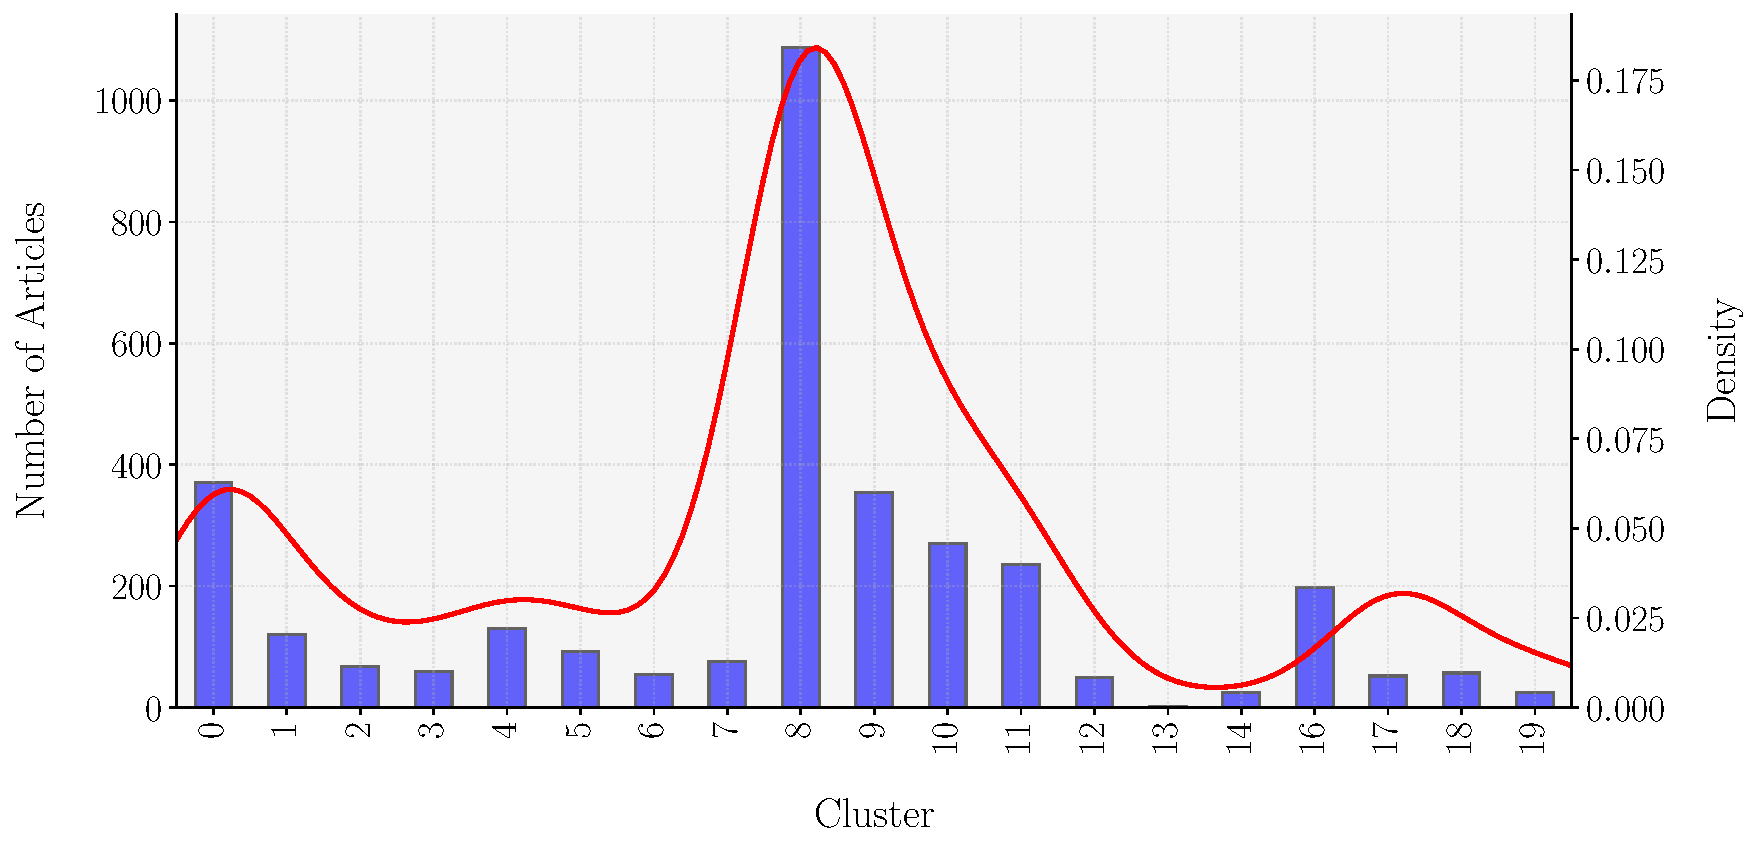
\includegraphics[scale=0.48]{/Users/jesusvillotamiranda/Library/CloudStorage/OneDrive-UniversidaddeLaRioja/CEMFI/Rest/__Second_year__/MasterThesis/__Output/LLAMA_Cluster_Distribution.pdf}
        \label{fig:all_data}
    \end{subfigure}

    % Lower plots
    \begin{subfigure}[b]{0.32\textwidth}
        \caption{Training data ($\D^{tr}$)}
        \centering
        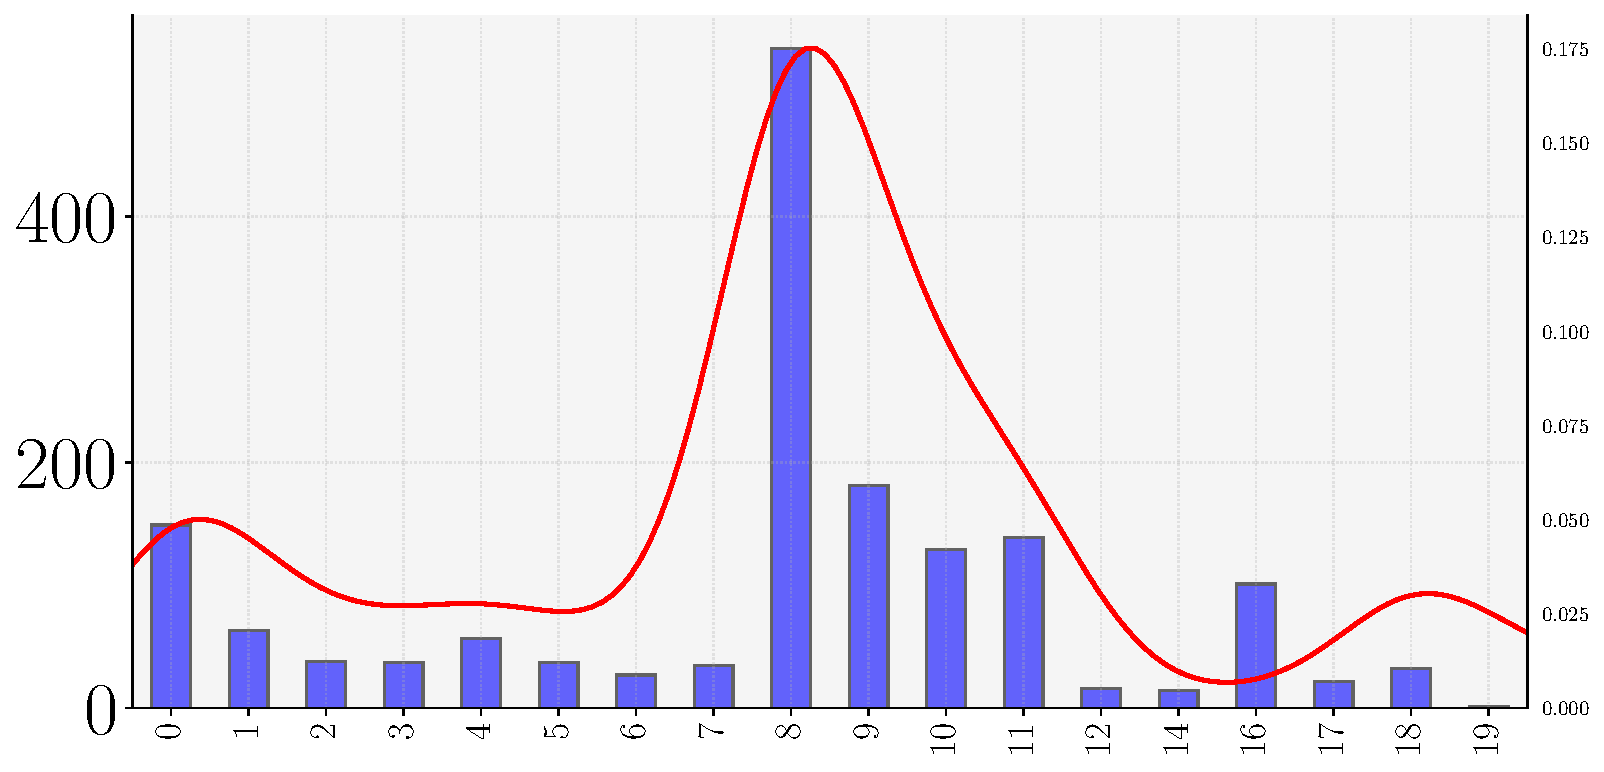
\includegraphics[width=\textwidth]{/Users/jesusvillotamiranda/Library/CloudStorage/OneDrive-UniversidaddeLaRioja/CEMFI/Rest/__Second_year__/MasterThesis/__Output/LLAMA_Cluster_Distribution_Train.pdf}
        \label{fig:train_data}
    \end{subfigure}
    \begin{subfigure}[b]{0.32\textwidth}
        \caption{Validation data ($\D^{val}$)}
        \centering
        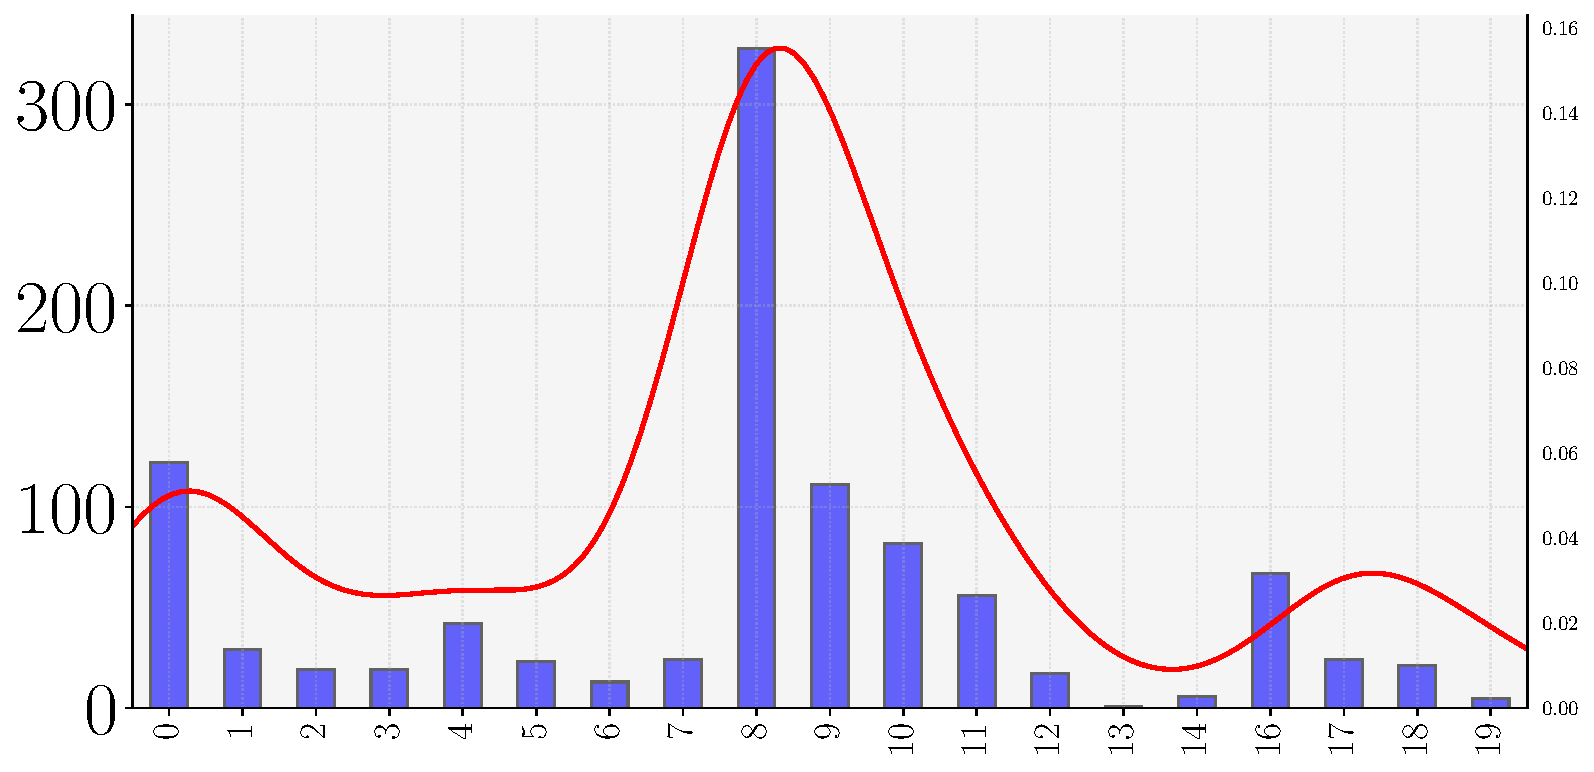
\includegraphics[width=\textwidth]{/Users/jesusvillotamiranda/Library/CloudStorage/OneDrive-UniversidaddeLaRioja/CEMFI/Rest/__Second_year__/MasterThesis/__Output/LLAMA_Cluster_Distribution_Validation.pdf}
        \label{fig:val_data}
    \end{subfigure}
    \begin{subfigure}[b]{0.32\textwidth}
        \caption{Test data ($\D^{test}$)}
        \centering
        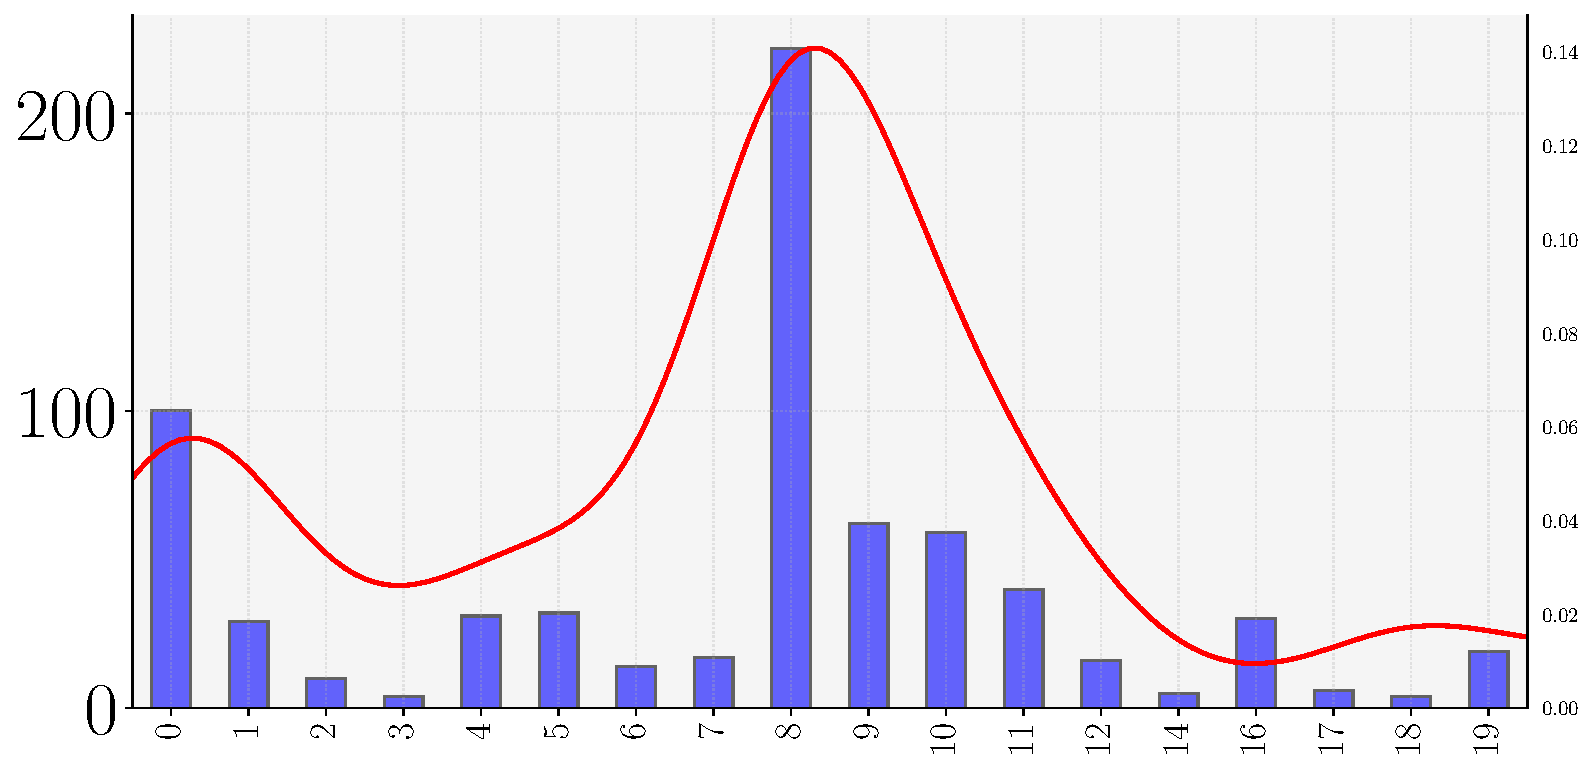
\includegraphics[width=\textwidth]{/Users/jesusvillotamiranda/Library/CloudStorage/OneDrive-UniversidaddeLaRioja/CEMFI/Rest/__Second_year__/MasterThesis/__Output/LLAMA_Cluster_Distribution_Test.pdf}
        \label{fig:test_data}
    \end{subfigure}
    \label{fig:LLM_cluster_distribution}
\subcaption*{\textit{Note: The upper plot shows the distribution of all the articles $i\in \mathcal D$ through the LLM clusters, while the lower plots show the distributions for the training ($\D^{tr}$), validation ($\D^{val}$), and test ($\D^{test}$) articles respectively.}}
\end{figure}
%----------------------------------------------------
%----------------------------------------------------


In the same fashion as before, we can plot the distribution of cluster-average Sharpe Ratios for each data split. Different from before, all distributions are left-skewed. The train split's distribution has fat tails which severely contrasts with the light-tailed distribution of the validation sample. In the test data, we observe a bell-shaped distribution with some accumulation of mass at high $SR$s (between 5 and 15).
%----------------------------------------------------
\begin{figure}[H]
  \centering
  \caption{Distribution  of Cluster-Average Sharpe Ratios $(\overline{SR}_g)$ by Split}
  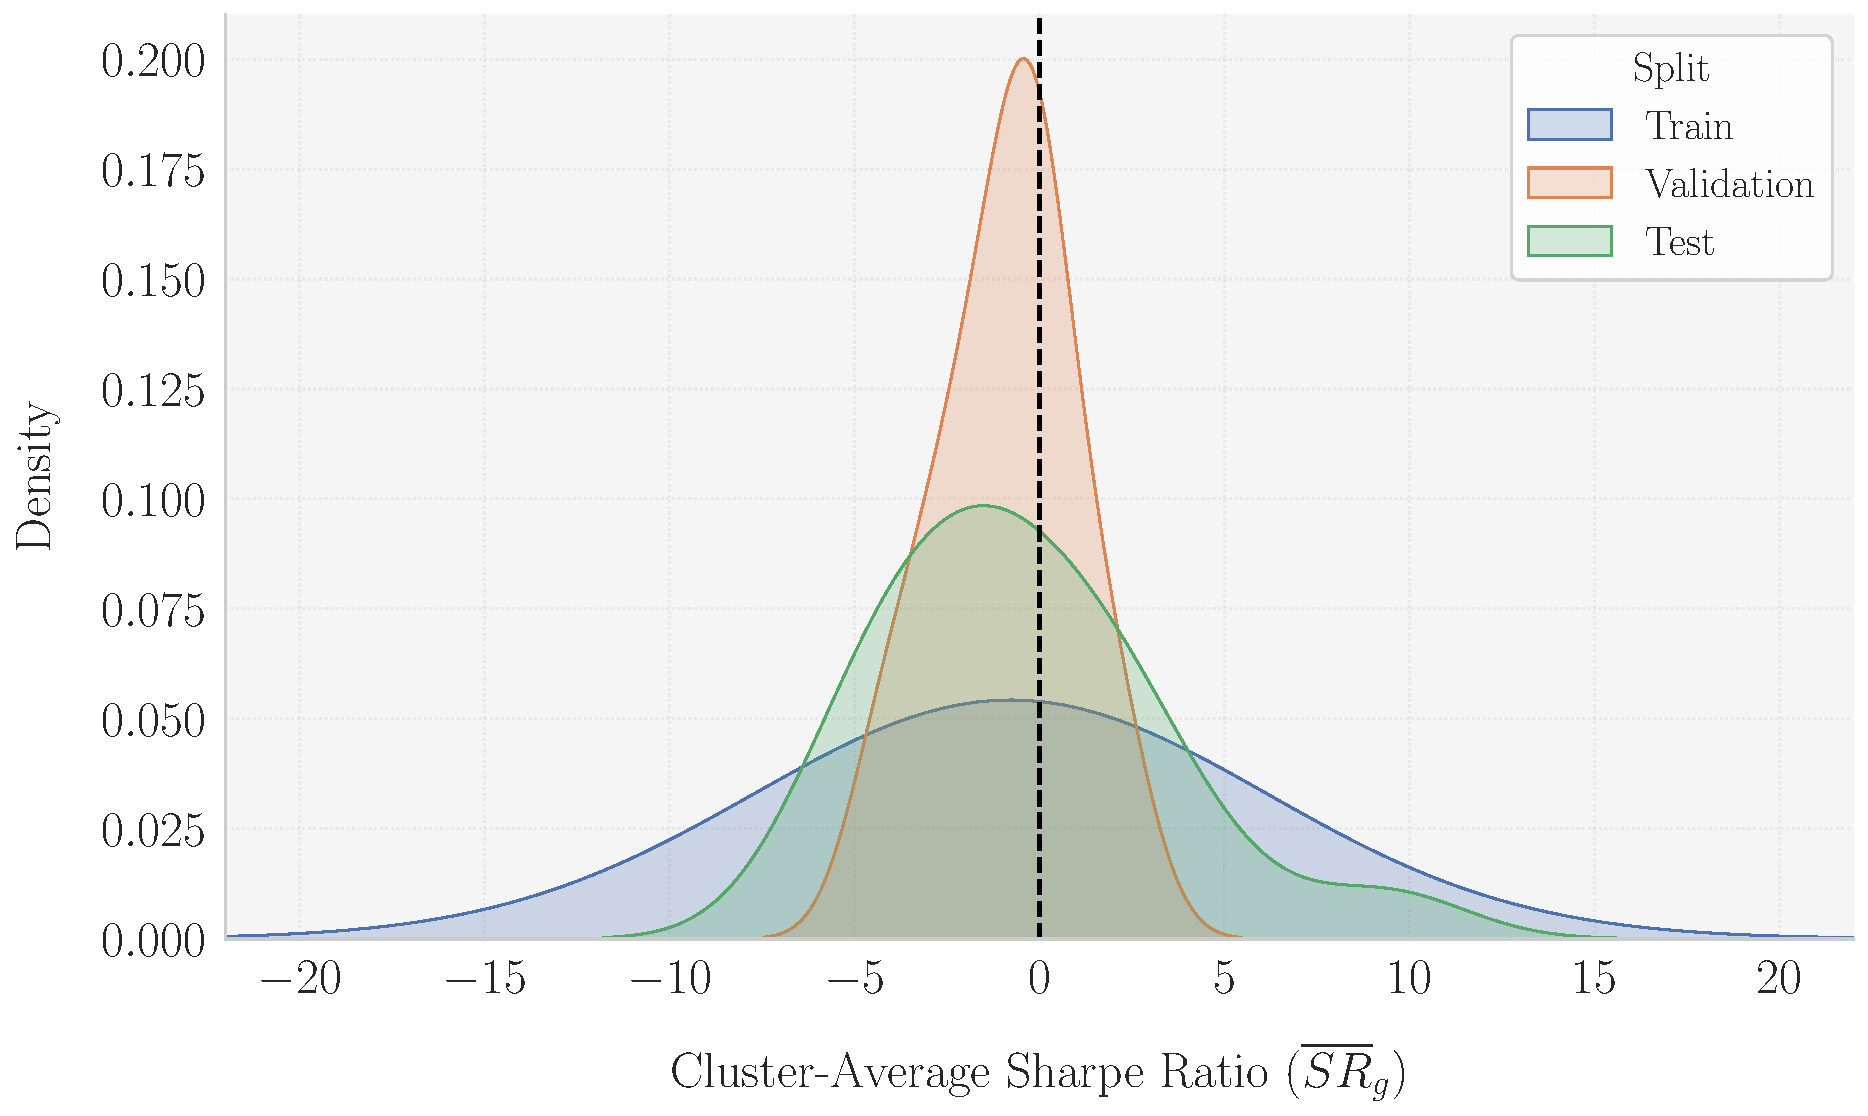
\includegraphics[scale=0.5]{/Users/jesusvillotamiranda/Library/CloudStorage/OneDrive-UniversidaddeLaRioja/CEMFI/Rest/__Second_year__/MasterThesis/__Output/LLAMA_Cluster-Avg_SR_Distribution.pdf}
\end{figure}
%----------------------------------------------------

\subsubsection{Trading Strategy using LLM-based clusters}

\hspace{0.5cm} The advantage of clustering with an LLM is that signals become cleaner and more interpretable. The selection of clusters by the \textit{Greedy} algorithm is highly correlated with the direction of the shocks. Intuitively, the stock price of a firm that is negatively affected by a shock is expected to go down and vice versa.

\mx 
Looking at \cref{tab:LLM_cluster_mapping_extended} we can clearly see that both algorithms go short on articles classified as policy shocks independently of the direction (positive or negative). Both algorithms go long on the famous cluster 8, which, as we discussed above, concentrates about 1/3 of the news articles. This cluster contains articles categorized as undergoing financial minor and positive shocks.
Counterintuitively, both algorithms go long on negative major demand shocks and they go short on positive major demand shocks. 



%----------------------------------------------------
\inserthere{tab:LLM_cluster_mapping_extended}

\begin{table}[H]
\caption{Mapping of LLM-based clusters to Trading Signals}
\centering
%{\footnotesize
\begin{tabular}{C{1cm}lcc}
\hline \Xhline{2\arrayrulewidth}
%\rowcolor{gray!10}
 \multicolumn{2}{c}{\textbf{Cluster}} & \textbf{Greedy} & \textbf{Stable} \\ \hline \Xhline{2\arrayrulewidth} 
0 & {(demand, minor, positive)} &  &  \\ \hline
1 & {(demand, minor, negative)} &  & \textcolor{darkred}{\textsc{short}} \\ \hline
2 & {(demand, major, positive)} & \textcolor{darkred}{\textsc{short}} & \textcolor{darkred}{\textsc{short}} \\ \hline
3 & {(demand, major, negative)} & \textcolor{darkgreen}{\textsc{long}} & \textcolor{darkgreen}{\textsc{long}} \\ \hline
\Xhline{2\arrayrulewidth}
4 & {(supply, minor, positive)} & \textcolor{darkgreen}{\textsc{long}} &  \\ \hline
5 & {(supply, minor, negative)} & \textcolor{darkred}{\textsc{short}} &  \\ \hline
6 & {(supply, major, positive)} & \textcolor{darkgreen}{\textsc{long}} &  \\ \hline
7 & {(supply, major, negative)} & \textcolor{darkred}{\textsc{short}} &  \\ \hline
\Xhline{2\arrayrulewidth}
8 & {(financial, minor, positive)} & \textcolor{darkgreen}{\textsc{long}} & \textcolor{darkgreen}{\textsc{long}} \\ \hline
9 & {(financial, minor, negative)} &  & \textcolor{darkred}{\textsc{short}} \\ \hline
10 & {(financial, major, positive)} & \textcolor{darkgreen}{\textsc{long}} &  \\ \hline
11 & {(financial, major, negative)} & \textcolor{darkred}{\textsc{short}} &  \\ \hline
\Xhline{2\arrayrulewidth}
12 & {(technology, minor, positive)} & \textcolor{darkgreen}{\textsc{long}} &  \\ \hline
13 & {(technology, minor, negative)} &  &  \\ \hline
14 & {(technology, major, positive)} & \textcolor{darkred}{\textsc{short}} &  \\ \hline
15 & {(technology, major, negative)} &  &  \\ \hline
\Xhline{2\arrayrulewidth}
16 & {(policy, minor, positive)} & \textcolor{darkred}{\textsc{short}} & \textcolor{darkred}{\textsc{short}} \\ \hline
17 & {(policy, minor, negative)} & \textcolor{darkred}{\textsc{short}} & \textcolor{darkred}{\textsc{short}} \\ \hline
18 & {(policy, major, positive)} & \textcolor{darkred}{\textsc{short}} & \textcolor{darkred}{\textsc{short}} \\ \hline
19 & {(policy, major, negative)} & \textcolor{darkred}{\textsc{short}} & \textcolor{darkred}{\textsc{short}} \\ \hline
\Xhline{2\arrayrulewidth}
\end{tabular}
%}
\vspace{0.5cm}
\subcaption*{\textit{
Note: Mapping of LLM-based clusters to their Trading Signal \textsc{(long/short)} for the two proposed cluster-selection algorithms (Greedy and Stable). The Greedy algorithm longs (shorts) clusters that maximize (minimize) the cluster-average-$SR$ in the validation sample subject to a positivity (negativity) constraint, while the Stable algorithm longs (shorts) clusters that minimize the rank difference between the training and validation rankings of the cluster-average-$SR$'s subject to a positivity (negativity) constraint, which is now imposed on both sample splits. In both algorithms, the cardinality of each leg is upper-bounded by a hyperparameter $\theta$. Each cluster corresponds to a type of news-implied firm-specific shock identified by our LLM according to the function calling schema.
}}
\label{tab:LLM_cluster_mapping_extended}
\end{table}
%----------------------------------------------------

\mx 
In \cref{fig:LLM_portfolio_returns} we plot the cumulative returns of the portfolio based on LLM clustering ($\mathcal P_{LLM}$). As before, both algorithms perform really well on ``seen'' data. However, different from before, the \textit{Greedy} algorithm works well also on the Training Split (which it was not trained on). More importantly, both algorithms do a great job in the test data. As we can see, both are able to achieve a consistent profile of earnings through the split. 
%In this case, the correlation of the trading signals generated by both algorithms is higher (0.693)

\mx 
The summary statistics of the portfolio are provided in \cref{tab:LLM_portfolio_statistics}, where we see confirmed the fact that both algorithms excel at generating profits even out of sample. 

%----------------------- PLOT ----------------------
\begin{figure}[H]
  \centering
    \caption{Cumulative Returns of $\mathcal P_{LLM}$ across data splits}
  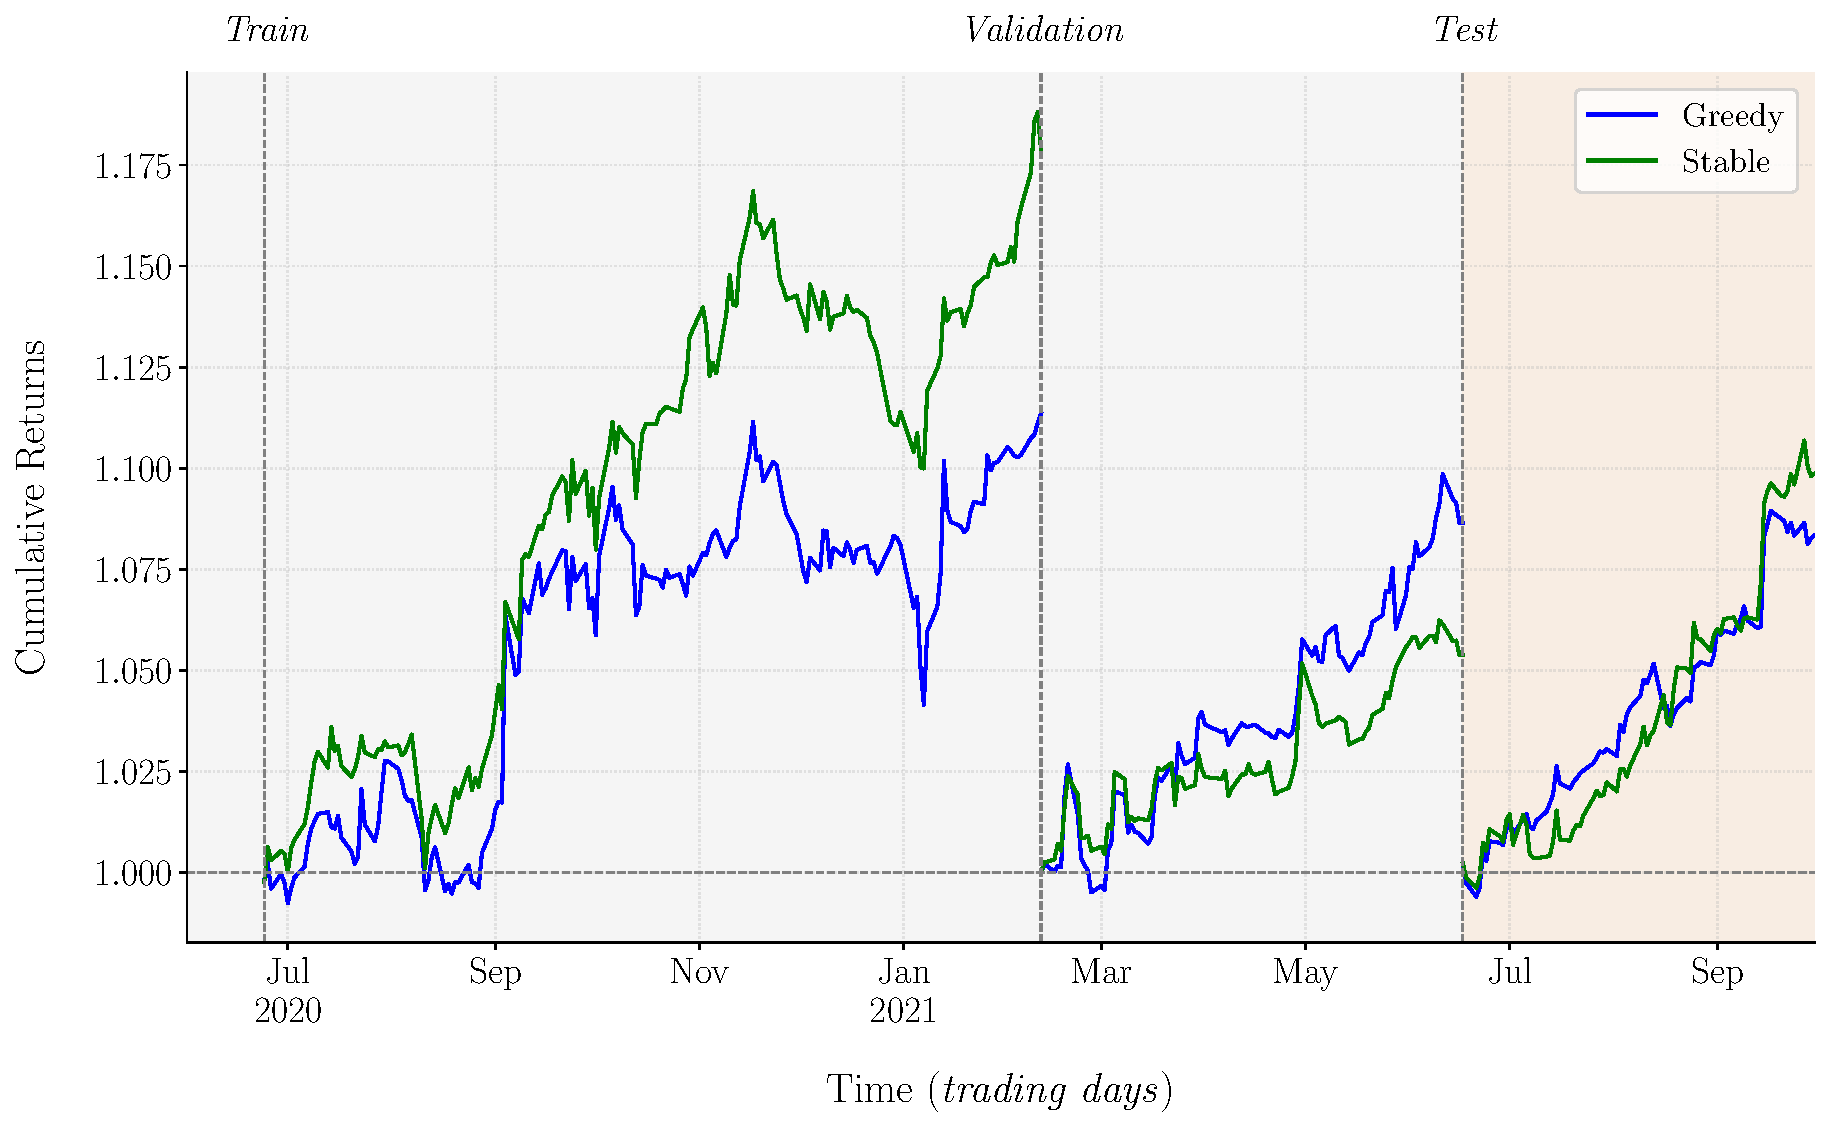
\includegraphics[scale=0.58]{/Users/jesusvillotamiranda/Library/CloudStorage/OneDrive-UniversidaddeLaRioja/CEMFI/Rest/__Second_year__/MasterThesis/__Output/LLAMA_Portfolio_Cum_Returns_(L=4,theta=0.5k).pdf}
  \subcaption*{\textit{Note: The holding period of the beta-neutral strategies is set to $L=4$ trading days and the number of traded clusters is  $\theta=\integer{0.5k}=10$, as now we have $k=20$ clusters. The selection criteria for these parameters is based on maximizing the Sharpe Ratios of the train and validation samples. }}
  \label{fig:LLM_portfolio_returns}
\end{figure}
%----------------------------------------------------


%\blue{
%\begin{itemize}
% \item The cumulative returns of the portfolio obtained by applying our selection algorithms to the LLM clusters is plotted in \cref{fig:LLM_portfolio_returns}. As we can see, different from before, now the portfolio does surprisingly well on unseen data (test set). 
%  \item The visual results of the plot, are confirmed by the statistics of the portfolio, which we can see in \cref{tab:LLM_portfolio_statistics}.
%  \item The correlation betweent he trading signals generated by the greedy and stable algorithm are, in this case, 0.693604
%\end{itemize}
%
%}

%--------------------- TABLE ------------------------
\inserthere{tab:LLM_portfolio_statistics}

\begin{table}[H]
    \caption{Statistics of $\mathcal{P}_{LLM}$ across data splits}
    \centering
    \renewcommand{\arraystretch}{0.8}
    \begin{tabular}{cccccc}
        \hline \Xhline{2\arrayrulewidth}
%        \rowcolor{gray!10}
        \textbf{Split} & \textbf{Algorithm} & \textbf{Cum. Return} & \textbf{Avg. Return} & \textbf{St. Deviation} & \textbf{Sharpe Ratio} \\
%        \rowcolor{gray!10}
        & & & \textit{(daily)} & \textit{(daily)} & \textit{(annual)} \\
		\hline \Xhline{2\arrayrulewidth}
        \multirow{2}{*}{All}       & \textit{Greedy} & 1.311 & 0.082 & 0.006 & 2.17 \\        & \textit{Stable} & 1.365 & 0.095 & 0.005 & 2.78 \\         \hline          \multirow{2}{*}{Train}       & \textit{Greedy} & 1.113 & 0.065 & 0.007 & 1.44 \\        & \textit{Stable} & 1.179 & 0.100 & 0.006 & 2.53 \\         \hline          \multirow{2}{*}{Validation}       & \textit{Greedy} & 1.086 & 0.093 & 0.005 & 2.86 \\        & \textit{Stable} & 1.054 & 0.059 & 0.004 & 2.16 \\         \hline          \multirow{2}{*}{Test}       & \textit{Greedy} & 1.083 & 0.105 & 0.004 & 4.30 \\        & \textit{Stable} & 1.099 & 0.124 & 0.004 & 4.38 \\         \hline \Xhline{2\arrayrulewidth}
    \end{tabular}
    \label{tab:LLM_portfolio_statistics}
\vspace{0.5cm}
\subcaption*{\textit{Note: Portfolio statistics of the trading strategy applied to the LLM clusters. The statistics provided are: Cumulative Return, Average Return, Standard Deviation and Sharpe Ratio, which have been computed in accordance to the formulas provided in the text. Such statistics are provided for both cluster-selection algorithms: Greedy and Stable. The Greedy algorithm longs (shorts) clusters that maximize (minimize) the cluster-average-$SR$ in the validation sample subject to a positivity (negativity) constraint, while the Stable algorithm longs (shorts) clusters that minimize the rank difference between the training and validation rankings of the cluster-average-$SR$'s subject to a positivity (negativity) constraint, which is now imposed on both sample splits. In both algorithms, the cardinality of each leg is upper-bounded by a hyperparameter $\theta$. 
The holding period of the beta-neutral positions is set to $L$ = 4 trading days and the number of traded clusters is, $\theta = 0.5k=13$ as there are $k^*=26$ KMeans clusters of article embeddings. The selection criteria for these hyperparameters ($L,\theta$) is based on maximizing the Sharpe Ratios of the train and validation samples.
}}
\end{table}
%----------------------------------------------------
